\newpage
\section{Using Pleiades images in \app and \mont}\label{sec:pleiades}

The typical Pleiades product is a pansharpened image of 40 000 by 40
000 pixels large, with 4 spectral bands, but one can even order larger
mosaics, whose size can be even larger, with hundreds of thousands of
pixels in each dimension.

To allow easier storage and transfer of such products, the standard
image file format is JPEG2000, which allows to achieve high
compression rates. The counterpart of these better storage and
transfer performances is that the performance of pixels accesses
within those images may be poorer than with an image format without
compression, and even more important, the cost of accessing pixels is
not uniform: it depends on where are the pixels you are trying to
access, and how they are spatially arranged.

To be more specific, Pleiades images are internally encoded into 2048
per 2048 pixels tiles (within the JPEG2000 file). These tiles
represent the atomic decompression unit: if you need a single pixel
from a given tile, you still have to decode the whole tile to get
it. As a result, if you plan to access a large amount of pixels within
the image, you should try to access them on a per tile basis, because
anytime you ask for a given tile more than once, the performances of
your processing chains drop.

What does it mean ? In OTB, the streaming (on the flow) pipeline
execution will try to stay synchronised with the input image tiling
scheme to avoid decoding the same tile several time. But you may know
that in the OTB world, one can easily chain numerous processing, some
them enlarging the requested region to process the output - like
neighbourhood based operators for instance - or even completely change
the image geometry - like ortho-rectification for instance. And this
chaining freedom is also at the heart of Monteverdi. In short, it is
very easy to build a processing pipeline in OTB or chain of modules in
Monteverdi that will get incredibly bad performances, even if the OTB
back-end does its best to stay in tune with tiles. And here, we do not
even speak of sub-sampling the whole dataset at some point in the
pipeline, which will lead to even more incredibly poor performances,
and is however done anytime a viewer is called on a module output in
Monteverdi.

So, can \mont or \app open and process Pleiades images ? Fortunately
yes. \mont even takes advantage of JPEG2000 ability to generate
coarser scale images for quick-look generation for visualisation
purposes. But to ease the use of Pleiades images in \mont, we chose to
open them in a separate data type, and to lock the use of most of
modules for this data type. It can only be used in the Viewer module
and a dedicated module allowing to uncompress a user-defined part of a
Pleiades image to disk. One can still force the data type during the
opening of the image, but this is not advised: the advised way to use
the other modules with Pleiades data is to first uncompress to disk
your area of interest, and then open it again in Monteverdi (careful,
you may need a lot of disk space to do this). As for the applications,
they will work fine even on JPEG2000 Pleiades data, but keep in mind
that a performance sink might show depending on the processing you are
try to achieve. Again, the advised way of working would be to
uncompress your area of interest first and then work with the
uncompressed file, as you used to with other data.

A final word about metadata: \app and \mont can read the Dimap V2
(note that we also read the less non-official Dimap V1.1 format)
metadata file associated with the JPEG2000 file in the Pleiades
product. It reads the RPC localisation model for geo-coding and the
information needed to perform radiometric calibration. These metadata
will be written in an associated geom file when uncompressing your
area of interest to disk, so that both \mont and \app will be able to
retrieve them, even for images extracts.

\subsection{Opening a Pleiades image in \mont}

Opening a Pleiades image in \mont is not different from opening other
kind of dataset: use the \textit{Open Dataset} item from the
\textit{File} menu, and select the JP2 file corresponding to you image
using the file browser.

\begin{figure}
  \center
  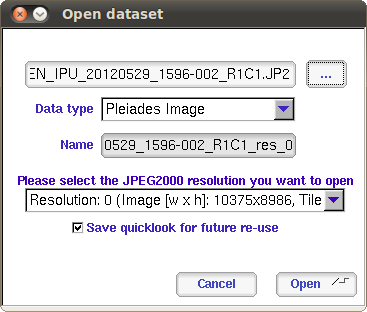
\includegraphics[width=0.4\textwidth]{../Art/MonteverdiImages/pleiades_open.png}
  \itkcaption[Monteverdi Pleiades image opening]{Dialog window when opening a pleiades image in Monteverdi}
  \label{fig:pleiades_open}
\end{figure}

Figure~\ref{fig:pleiades_open}, page~\pageref{fig:pleiades_open} shows
the dialog box when opening a Pleiades image in \mont.

\subsection{Viewing a Pleiades image in \mont}

\subsection{Handling mega-tiles in \mont}

\subsection{Partial uncompressing of Pleiades images in \mont}

\subsection{Other processing of Pleiades images with \mont}

\subsection{Processing of Pleiades images with \app}
